% !TEX root = ../main.tex

% 封面页
% 参考：https://zh.wikibooks.org/wiki/LaTeX/%E7%94%9F%E6%88%90%E5%B0%81%E9%9D%A2%E5%92%8C%E6%A0%87%E9%A2%98

% 标题
\newcommand{\HRule}{\rule{\linewidth}{0.5mm}} % \rule{\linewidth}{0.5mm} 表示创建一条宽度为 \linewidth、厚度为 0.5mm 的水平线。

% 日期
\renewcommand{\today}{\DTMtoday} % 使用 datetime2 提供的今日日期命令
%\renewcommand{\today}{January 21, 2025} % 固定日期

\begin{titlepage}
	
%	% 经典模版，参考如上
%	\begin{center}
%		
%		% Upper part of the page
%%		
\includegraphics[width=0.5\textwidth]{logo}\\[1cm] % LOGO，通常为注释掉的
%		\textsc{\huge SYSU·SPA}\\[1.5cm]
%		\textsc{\LARGE A Note of Personal Project}\\[0.5cm]
%		
%		% Title
%		\HRule \\[0.4cm]
%		{ \Huge \bfseries Physics with Coding}\\[0.1cm]
%		\HRule \\[1.5cm]
%		
%		% Author and supervisor
%%		\begin{minipage}{0.4\textwidth}
%%			\begin{flushleft} \large
%%				\emph{\textbf{Author:}}\\
%%				John \textsc{Smith}
%%			\end{flushleft}
%%		\end{minipage}
%%		\begin{minipage}{0.4\textwidth}
%%			\begin{flushright} \large
%%				\emph{Supervisor:} \\
%%				Dr.~Mark \textsc{Brown}
%%			\end{flushright}
%%		\end{minipage}
%%		% 下面提供了一个简化版
%		\LARGE\emph{\textbf{copyright@pifuyuini}}
%		
%		\vfill
%		
%		% Bottom of the page
%		\Large\texttt{\textcolor{fgrayblue}{Programming instruction for undergraduate physics students.}}
%		
%		\hspace*{\fill}
%		
%		{\LARGE \today}
%		
%	\end{center}
	
	% 下面是另一个模版，通常为注释的，参考https://zhuanlan.zhihu.com/p/604236564（美化，封面1）
	
	% 通过这两个命令，页面会完全取消边距和段落首行缩进。这通常用于特殊格式的页面（如封面、图表页）或实现全屏显示的效果。
	\newgeometry{margin = 0in}
	\parindent=0pt
	
	% 插图
	\begin{figure}
		\centering
		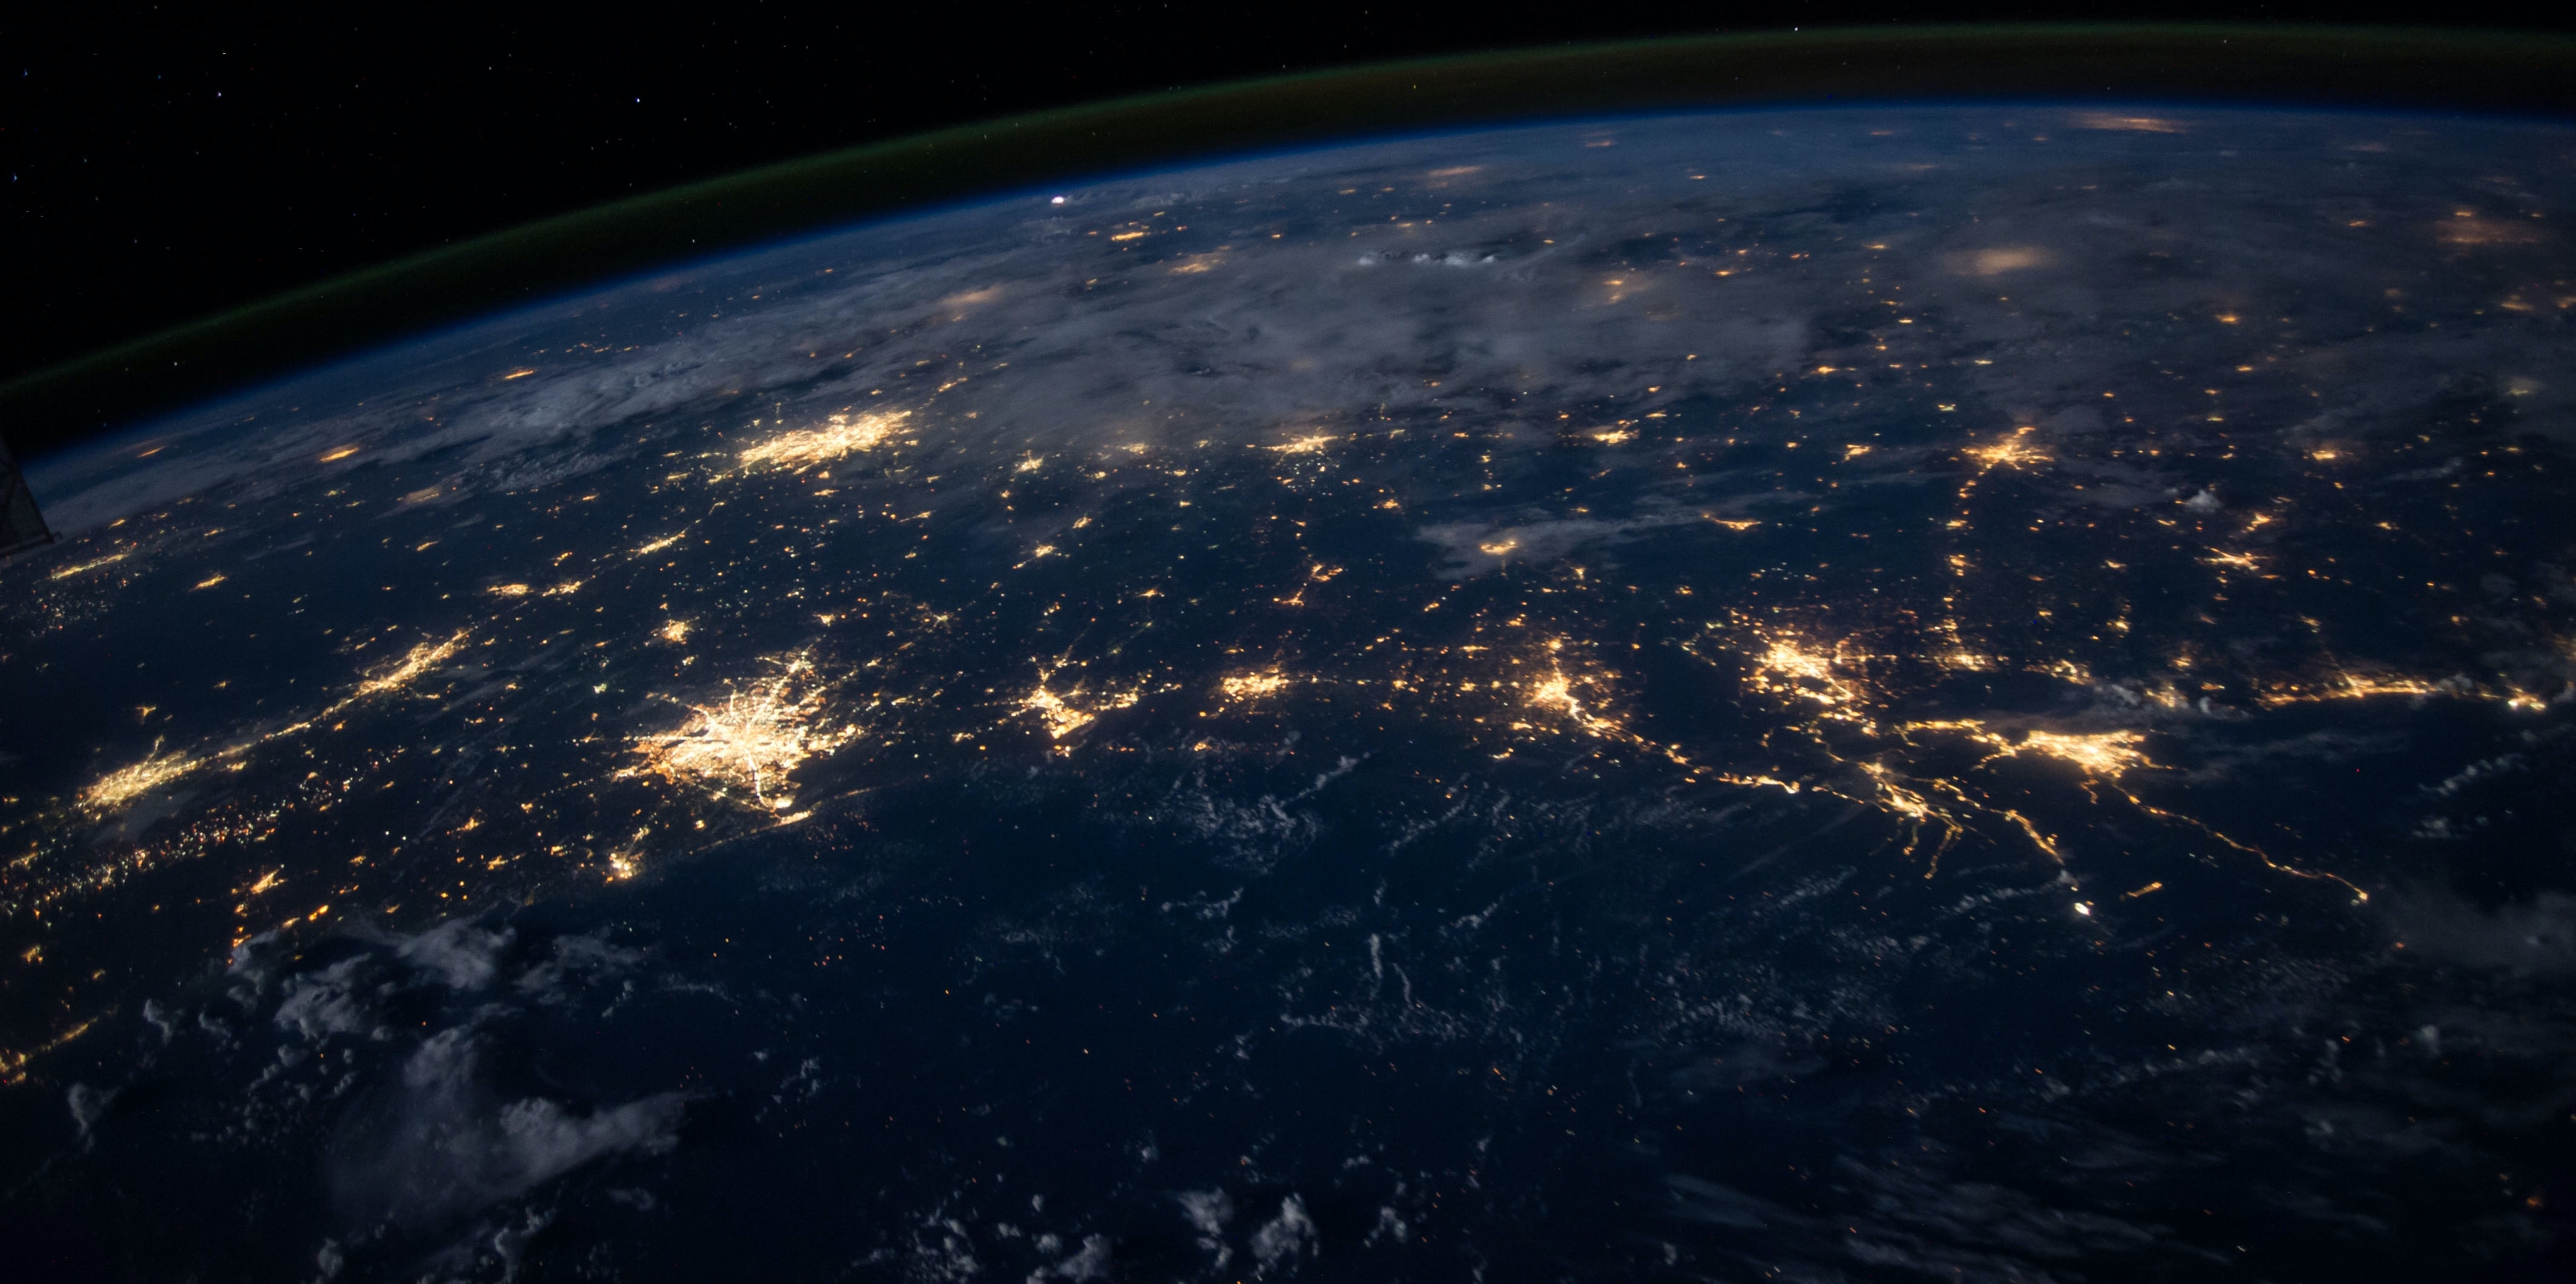
\includegraphics[width=\linewidth]{images/illustrations}
	\end{figure}
	
	\begin{flushright}
		% 标题
		{ \Huge \bfseries Physics with Coding} \hspace*{6em} \\[0.2cm]
		\rule{0.618\textwidth}{5pt} \hspace*{6em} \\[1cm]
		
		% 作者
		\LARGE\emph{\textbf{Copyright@pifuyuini}} \hspace*{4.2em}
		
	\end{flushright}
	
	% Bottom of the page
	\begin{center}
		\vfill
		
		\Large\texttt{\textcolor{fgrayblue}{Programming instruction for undergraduate physics students.}}
		
		\hspace*{\fill}
		
		{\LARGE \today}
		
		\hspace*{\fill}
	\end{center}
	
\end{titlepage}